\section{Auswertung}
\label{sec:Auswertung}

% \begin{figure}
%   \centering
%   \includegraphics{plots/plot.pdf}
%   \caption{Plot.}
%   \label{fig:plot}
% \end{figure}



% \begin{table}
%    % Notation :  {% nicht entfernen ist sehr wichtig sonst Fehler !!
% \parbox{0.48\textwidth}{% %Ermöglicht zwei Tabellen neben einander
%   \centering
%   \sisetup{round-mode = places , round-precision = 0,scientific-notation=fixed, fixed-exponent = 0}
%          %rundet Werte aus Stelle, Stelle = ,  macht einen bestimmten festen exponenten
%   \resizebox{\textwidth}{!}{%  % skaliert zu große Tabellen
%   \begin{tabular}{S@{${}\pm{}$} S} % fügt plus minus Fehler Schreibweise hinzu
%     \toprule
%      $\text{e}_b / \si{\milli\meter}$ &
%      $\text{d}_b /\si{\milli\meter} $ & $\text{f}_b / \si{\milli\meter} $\\
%     \midrule
%     \bottomrule
%   \end{tabular}
%   % }
%   \caption{Tabellenunterschrift}
%   \label{tab:tab}
% }
% % \end{table}
% % \begin{table}
% \parbox{0.48\textwidth}{%
%   \centering
%   \sisetup{round-mode = places , round-precision = 0,scientific-notation=fixed, fixed-exponent = 0}
%   % \resizebox{\textwidth}{!}{%
%   \begin{tabular}{S@{${}\pm{}$} S}
%     \toprule
%      $\text{e}_b / \si{\milli\meter}$ &
%      $\text{d}_b /\si{\milli\meter} $ & $\text{f}_b / \si{\milli\meter} $\\
%     \midrule
%     \bottomrule
%   \end{tabular}
%   % }
%   \caption{Tabellenunterschrift}
%   \label{tab:tab}
% }
% \end{table}
\subsection{Bestimmung der Auflösungszeit}
Um die optimale Verzögerungszeit zu finden, wurde  $T_\text{Vz}$ varriert und gegen die Anzahl an Startimpulsen pro 10\,s aufgetragen.\\
In Abb. \ref{fig:Verzoegerung} sind die Messwerte aus Tabelle \ref{tab:Verzoegerung} aufgetragen. Da kein scharfes Maximum zu erwarten war,
wurde ein Plateau gefittet und die Halbwertsbreibe bestimmt.\\
Die Fehler der Counts wird mit dem $\sqrt{N}$-Gesetz abgeschätzt.\\
Die maximale Anzahl an Counts $N_{\text{max}}=(232\pm15)$ wurde bei einer Verzögerungszeit von $T_\text{Vz}=4\,\text{ns}$ gemessen, weshalb diese
an der Verzögerungsleitung eingestellt wurde.
\begin{figure}
  \centering
  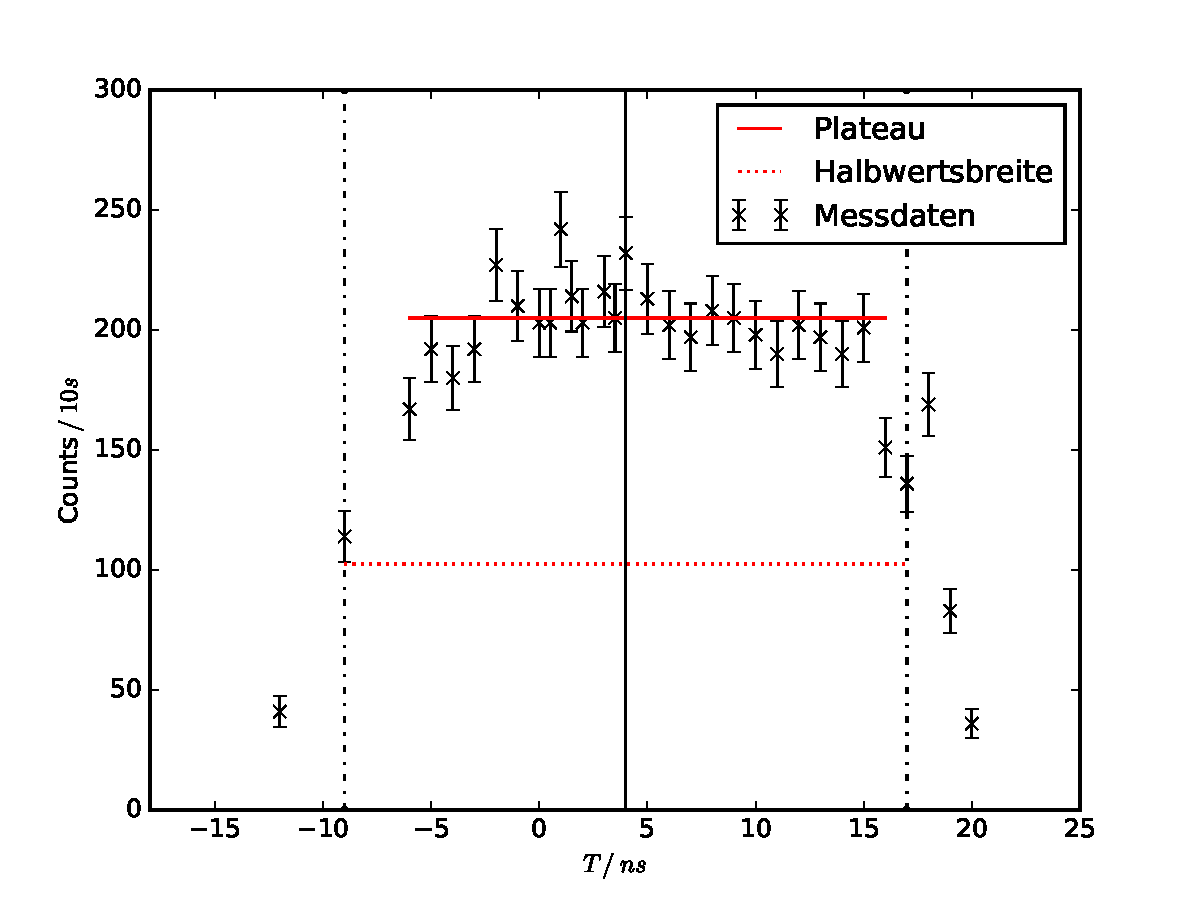
\includegraphics[width=0.8\textwidth]{plots/plotVerzoegerung.pdf}
  \caption{Messwerte und Fit des Plateaus zur Bestimmung der Verzögerungszeit.}
  \label{fig:Verzoegerung}
\end{figure}
Die in Abb. \ref{fig:Verzoegerung} bestimmte Halbwertsbreite entspricht der Auflösungszeit $\Delta t_{\text{k}}$
der Koinzidenzeinheit und ergibt sich aus den Längen der Diskriminatorimpulsen.
Hierbei sollte die Breite des Plateaus der Breite der Diskriminatorimpulsen entsprechen.\\
Die Halbwertsbreibe wurde Anhand
des Plots zu
\begin{equation*}
  \Delta t_{\text{k}}=(|-9|+|17|)\,\text{ns}=26\,\text{ns}
\end{equation*}
bestimmt.
Dies ist die Zeit, welche die untere Schranke bildet, in der zwei Impulse unterschieden werden können.\\
%Die Pulslänge des Diskriminators ist T$_\text{Puls}$ = 20 $\mu$s und somit geringer.
\begin{table}[H]
\centering
\caption{Messwerte zur Bestimmung der Auflösungszeit der Messapperatur}
\label{tab:Verzoegerung}
\begin{tabular}{c|c}
$T_{\text{VZ}}$ in ns& $N$\\
\hline
-12& 41\\
-9& 114\\
-6& 167\\
-5& 192\\
-4& 180\\
-3& 192\\
-2& 227\\
-1& 210\\
0& 203\\
0,5& 203\\
1& 242\\
1,5& 214\\
2& 203\\
3& 216\\
3,5& 205\\
4& 232\\
5& 213\\
6& 202\\
7& 197\\
8& 208\\
9& 205\\
10& 198\\
11& 190\\
12& 202\\
13& 197\\
14& 190\\
15& 201\\
16& 151\\
17& 136\\
18& 169\\
19& 83\\
20& 36\\
\end{tabular}
\end{table}
\subsection{Zeitkalibrierung der Messapperatur}
Um den Vielkanalanalysator zu kalibrieren werden mit Hilfe eines Doppelimpuls-Generators Impulse mit unterschiedlichem
zeitlichem Abstand eingelesen. Die belegten Kanäle sind in Tabelle \ref{tab:Kalibrierung} dargestellt und in Abbildung \ref{fig:Kalibrierung}
gegen die Impulsabstände aufgetragen.
\begin{table}[H]
\centering
\caption{Messwerte zur Bestimmung der Zeitkalibrierung der Messapperatur}
\label{tab:Kalibrierung}
\begin{tabular}{c|c}
Kanal&$T_{\text{VZ}}$ in $\upmu$s\\
\hline
23&	0.5\\
45&	1.0\\
68&	1.5\\
90&	2.0\\
112&	2.5\\
135&	3.0\\
157&	3.5\\
179&	4.0\\
202&	4.5\\
224&	5.0\\
246&	5.5\\
269&	6\\
291&	6.5\\
313&	7\\
336&	7.5\\
358&	8\\
381&	8.5\\
402&	9\\
443&	9.9\\
\end{tabular}
\end{table}
\begin{figure}
  \centering
  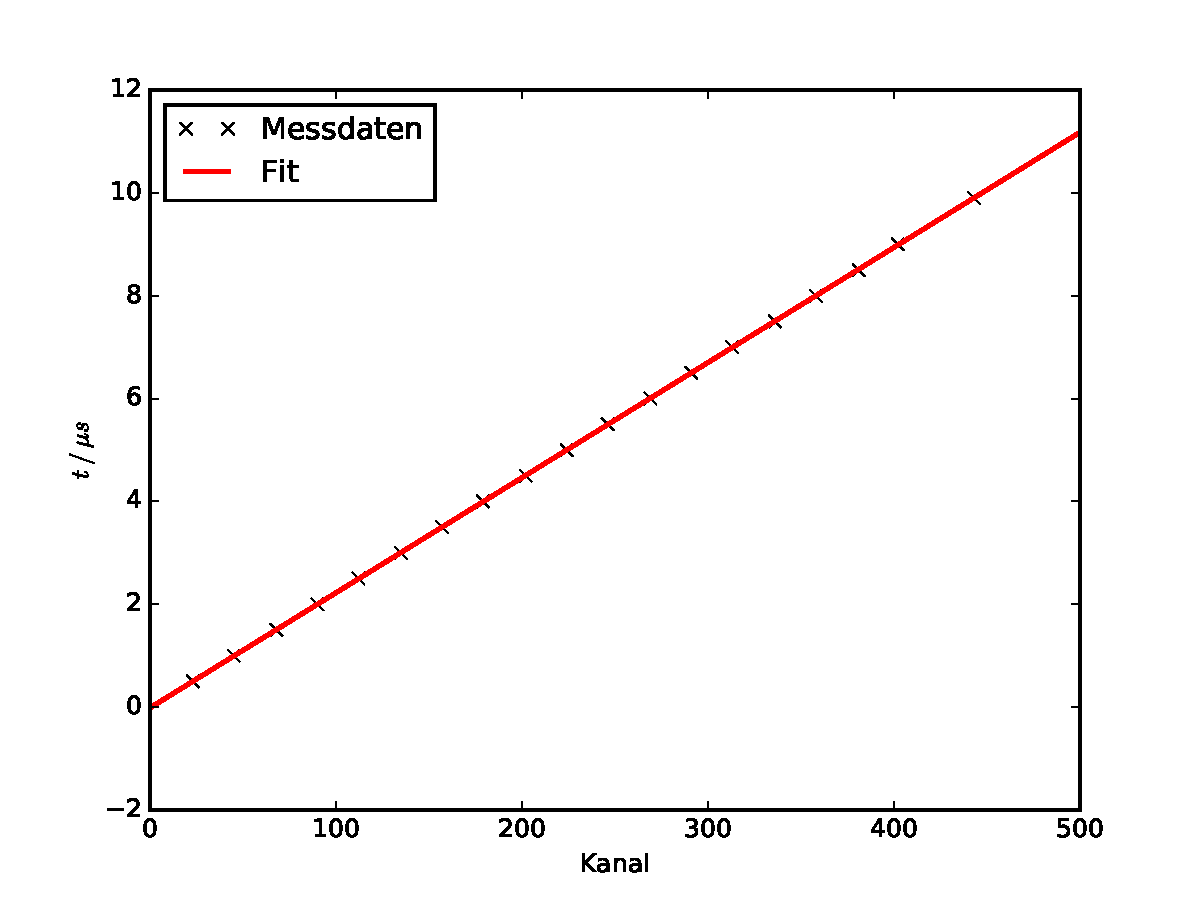
\includegraphics[width=0.8\textwidth]{plots/plotKanal.pdf}
  \caption{Messdaten und Fit zur Zeitkalibrierungder Apperatur.}
  \label{fig:Kalibrierung}
\end{figure}
Die lineare Regression der Form $f(x)=a\cdot x+b$ wird mit \cite{scipy} bestimmt und liefert für den Zusammenhang von Kanalnummer und Zeitabstand
\begin{equation}
  \Delta t =\left(0,02238 \pm 1,4\times 10^{-5}\right)\,\upmu\text{s}\cdot K + \left(-0,014 ± 0,003\right)\,\upmu\text{s}.
  \label{eq:KanalZeit}
\end{equation}
\subsection{Statistische Berechnung des Untergrundes}
Um den Untergrund zu bestimmen wird die Startimpulsrate
\begin{equation}
  n=\frac{N_{\text{Start}}}{t_{\text{Gesamt}}}=(25,05 \pm 0,01)\,\frac{1}{\symup{s}}
\end{equation}
aus der gesamten Messdauer $t_{\text{Gesamt}}= 83930$\,s und der Anzahl an Startimpulsen $N_{\text{Start}}= (2102553 \pm 1450)$ bestimmt.\\
Mit der poissionverteilten Wahrscheinlichkeit, dass n Teilchen während der Suchzeit $T_{\text{S}}= 11,2\,\upmu\text{s}$ den Tank
durchqueren kann die Anzahl an Fehlmessungen $N_{\text{F}}$ mit
\begin{equation}
  N_{\text{F}}=P\cdot N_{\text{Start}}=\frac{n\cdot T_{\text{S}}}{1!}e^{n\cdot T_{\text{S}}}\cdot N_{\text{Start}}
\end{equation}
berechnet werden.\\
Da diese Werte statistisch gleichverteilt sind kann die Untergrundrate pro Kanal mit
 \begin{equation}
   U=\frac{N_{\text{F}}}{512}
 \end{equation}
bestimmt werden.\\
Damit ergeben sich folgende Werte:
\begin{align*}
  P&=(0,0002805\pm0,0000002)\%\\
  N_{\text{F}}&=(589,8\pm0,8)\\
  U&=(1,152\pm0,002)\frac{1}{\text{Kanal}}
\end{align*}
\subsection{Bestimmung der Lebensdauer der Myonen}
Zur Bestimmung der Lebensdauer $\tau$ der Myonen wird die Anzahl an Stoppsignalen in den Kanalen des Vielkanalanalysators gespeichert.
In Abbildung \ref{fig:KanalCount} sind die Counts $N$ gegen die Kanäle aufgetragen.
\begin{figure}
  \centering
  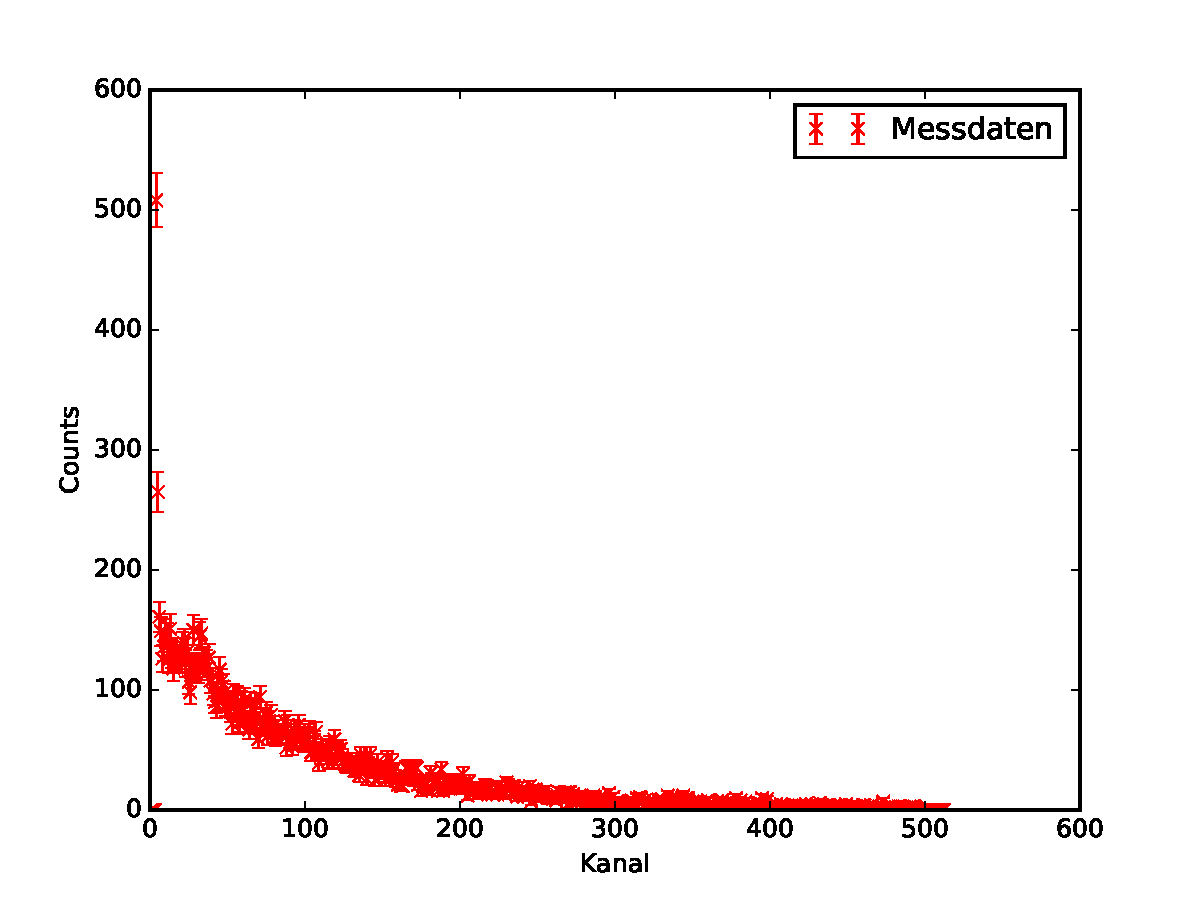
\includegraphics[width=0.8\textwidth]{plots/KanalCounts.pdf}
  \caption{Messdaten des Vielkanalanalysators.}
  \label{fig:KanalCount}
\end{figure}
Mit Gleichung \ref{eq:KanalZeit} wird aus den belegten Kanälen die Zeitdifferenz $\Delta t$ bestimmt und in Abbildung
\ref{fig:ZeitCounts} sowie \ref{fig:ZeitCountslin} aufgetragen.
\begin{figure}
  \centering
  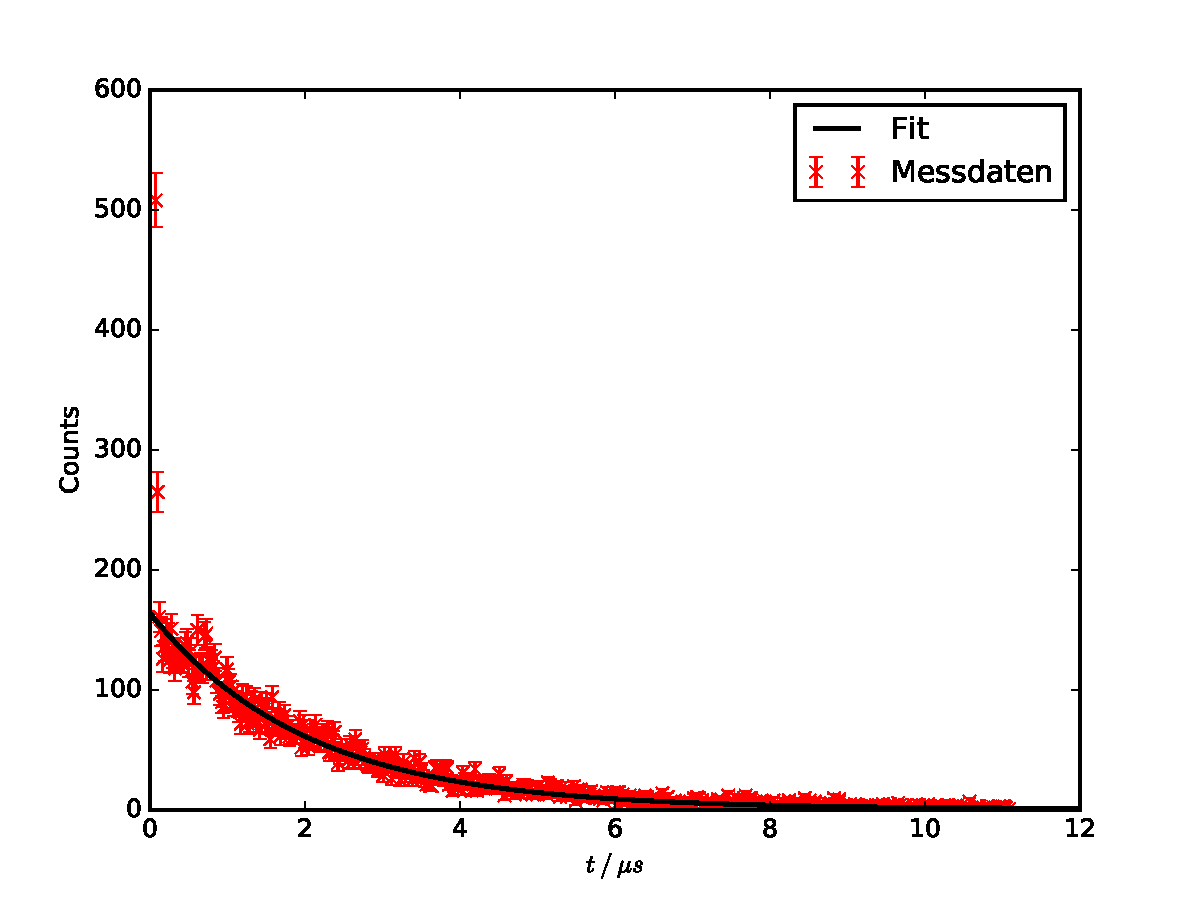
\includegraphics[width=0.8\textwidth]{plots/ZeitCounts.pdf}
  \caption{Zur Bestimmung der Lebensdauer wurden die gemessenen Counts gegen den berechneten
    zeitlichen Abstand aufgetragen und mit einer Exponentialfunktion gefittet.}
  \label{fig:ZeitCounts}
\end{figure}
\begin{figure}
  \centering
  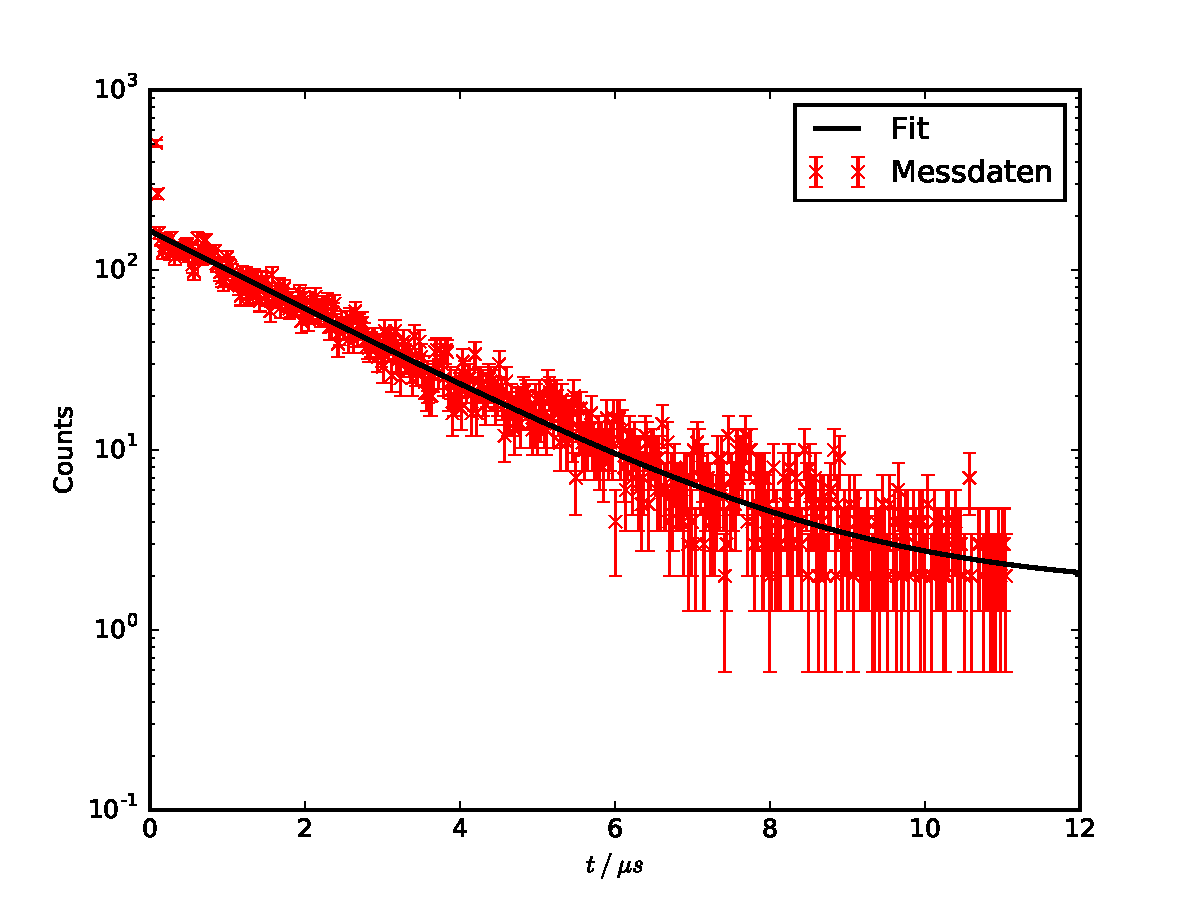
\includegraphics[width=0.8\textwidth]{plots/ZeitCountslinear.pdf}
  \caption{Der Übersichlichkeit halber wurden die Messdaten und der Fit aus Abb. \ref{fig:ZeitCounts} mit logarithmischer y-Achse dargestellt.}
  \label{fig:ZeitCountslin}
\end{figure}
Die Werte aus Abb. \ref{fig:ZeitCounts} wurden mit der Funktion
\begin{equation}
  N=N_0\cdot e^{-\lambda t}+U_{\text{fit}}
\end{equation}
gefittet.
Dabei ergeb sich für die Parameter folgende Werte:
\begin{align*}
  N_0&=(163 \pm 3)\\
  \lambda&=(0,495 \pm 0,009)\,\frac{1}{\upmu\text{s}}\\
  U_{\text{fit}}&=(0,8 \pm 0,2) \frac{1}{\text{Kanal}}
\end{align*}
Daraus lässt sich die Lebensdauer mit $\tau=\frac{1}{\lambda}$ zu
\begin{equation*}
  \tau=(2,02\pm0,04)\,\upmu\text{s}
\end{equation*}
bestimmen.
